\chapter{Exercise 5}
\label{cha:ugeopgave-5}

The purpose of the exercise is to get acquainted with input and window management in Glut and OpenGL. In particular we will work with mouse input, keyboard input, menus, multiple windows, logic operations, selection and picking.

\section{Part 1}
\label{sec:del-1}
According to mouse position information, pick function makes decision of the action that will be carried out.
Those actions are draw-triangle, draw-line, draw-rectangle, draw-point and drawing-mode.



\section{Part 2}
\label{sec:del-2}

\begin{itemize}
  \item When we clicked on a selectable item, picking function binds FBO objects and renders the scene on the FBO instead of default framebuffer.
  \item According to the mouse position when clicked, selected item information is extracted from FBO.
  \item Now we know which object is selected. The program flow goes on. We can do anything we want with selected object.
\end{itemize}


\section{Part 3}
\label{sec:del-3}

According to the recipe described in exercise sheet, I implement the Circuit diagram editor. I want to give my implementation details before giving a screenshot of a simple diagram that I create. \\
Move function can be used by user intuitively. User should left-click and hold on the object to be moved and should release the button when he or she has dragged the object to the desired place. Simply press on-hold left click,drag,release left-click.\\
Scale function can also be used intuitively. Once you click on an circuit item, if you move cursor further from the center of the item, item enlarges. On the other hand, if you move cursor closer to the center of the item, item shrinks. \\
Rotating may be a little bit tricky for the user at first glance. The mechanism works in this way: when user left-clicks o an item and holds on the button, if user moves cursor further from the center of the object, object rotates counter-clockwise around its center. If user moves the cursor further enough, the item makes a full 360 degrees turn. Therefore, user can give any angle to the item by rotating the item enough in counter-clockwise direction.\\
You can see a sample circuit diagram in Figure \ref{fig:5-3}


\begin{figure}[hp]
\centering
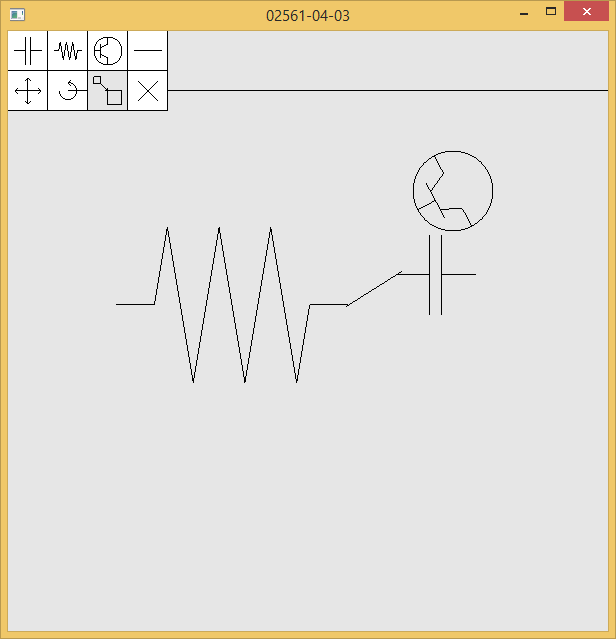
\includegraphics[width=8cm]{../Screenshots/ex-5/3.png}
\caption{A sample circuit diagram}
\label{fig:5-3}
\end{figure}



%%% Local Variables:
%%% mode: latex
%%% TeX-master: "report_main"
%%% End: 